\section{Rancangan}

Seperti yang telah dijelaskan pada \ref{subsection:alternatif-solusi}, solusi yang dipilih adalah membuat sistem dengan mengkombinasikan \textit{in-memory key-value store} dan menggunakan RocksDB sebagai \textit{persistent database}. Replikasi dan \textit{erasure coding} hanya dilakukan pada data persisten yang disimpan pada \textit{database} tersebut.

\subsection{Rancangan Struktural}
\label{subsection:rancangan-struktural}

Kebutuhan fungsional dan non-fungsional dipetakan pada struktur sistem yang diimplementasikan sebagai kumpulan komponen. Komponen didefinisikan sebagai sebuah unit fungsional yang berdiri sendiri dan dapat disusun. Beberapa komponen disusun secara hierarkis dan membentuk subsistem yang mewakili domain tanggung jawab tertentu dalam sistem. Setiap komponen dirancang untuk memenuhi tujuan spesifik berdasarkan kebutuhan sistem. Detail terkait setiap komponen ini dapat dilihat pada bagian \ref{subsection:detail-komponen}.

\subsection{Node}
\label{subsection:node}

\textit{Node} adalah satuan fungsional utama yang berperan sebagai entitas dalam sistem \textit{database} terdistribusi yang dikembangkan. Dalam eksperimen ini, \textit{Node} berfungsi sebagai \textit{key-value store}. Sesuai dengan perancangan pada bagian \ref{subsection:rancangan-struktural}, \textit{Node} dibangun secara modular dengan beberapa komponen yang tergabung dalam beberapa subsistem.

% Secara umum, struktur \textit{Node} terdiri dari:

% \begin{enumerate}
%     \item Subsistem penyimpanan: Subsistem ini bertanggung jawab untuk fungsionalitas \textit{key-value store} dalam sebuah \textit{Node}. Subsistem ini akan terdiri atas komponen \textit{in-memory store}, \textit{persistent store}, dan \textit{transaction log}. Subsistem ini juga mengkonfigurasi \textit{Node} untuk menggunakan replikasi atau \textit{erasure coding}.
%     \item Subsistem kontrol: Subsistem ini bertanggung jawab mengelola transaksi dan konsistensi antar-\textit{Node}. Pengelolaan tersebut dilakukan dengan mengaplikasikan algoritma konsensus untuk menjaga konsistensi data antar-\textit{Node}. Subsistem ini juga bertanggung jawab untuk melakukan \textit{recovery} data dari \textit{transaction log} jika terjadi kegagalan pada \textit{Node}.
%     \item Komponen HTTP \textit{server}: Komponen ini berperan sebagai antarmuka komunikasi antara \textit{client} dan \textit{Node}.
%     \item Komponen komunikasi antar-\textit{Node}: Komponen ini berfungsi untuk mengelola komunikasi antar-\textit{Node} dalam sistem terdistribusi. Komponen ini juga bertanggung jawab untuk mendistribusikan data ke \textit{Node} lain.
% \end{enumerate}

Merujuk analisis kebutuhan sistem pada bagian \ref{subsection:analisis-permasalahan}, \textit{Node} memenuhi kebutuhan 1 dan 2, yaitu:

\begin{enumerate}
    \item Sistem harus dapat mensimulasikan kondisi \textit{database} terdistribusi yang menggunakan replikasi ataupun \textit{erasure coding}.
    \item Sistem harus dapat menyimpan data secara \textit{persistent} untuk mensimulasikan kegagalan dan pemulihan.
\end{enumerate}

Sedangkan merujuk kebutuhan fungsional dan non-fungsional pada bagian \ref{subsection:system-requirements}, \textit{Node} memenuhi kebutuhan fungsional F-1, F-2, F-4, F-5, F-6, F-7, F-8, dan F-11 serta non-fungsional NF-1, NF-2, NF-3, dan NF-4.

\subsubsection{Data Collector}
\label{subsubsection:data-collector}

\textit{Data Collector} adalah satuan fungsional yang bertugas untuk melakukan \textit{request} dan transaksi pada sistem untuk mengumpulkan data eksperimen. \textit{Data Collector} ini memiliki fitur yang memungkinkan variasi dalam ukuran data, jumlah transaksi, dan pengukuran \textit{response time} untuk operasi. Selain itu, komponen ini juga dilengkapi dengan otomatisasi untuk menjalankan eksperimen berulang kali untuk mendapatkan data yang representatif dari eksperimen.

Secara umum, struktur \textit{Data Collector} terdiri dari:

% \begin{enumerate}
%     \item Komponen testing: Komponen ini bertanggung jawab untuk melakukan \textit{request} dan transaksi pada sistem.
%     \item Komponen \textit{logging} dan \textit{tracing}: Komponen ini mengelola pencatatan dan pelacakan operasi yang dilakukan oleh sistem secara keseluruhan.
%     \item Komponen \textit{reporting}: Komponen ini bertanggung jawab untuk mengumpulkan dan menyajikan hasil eksperimen dalam bentuk laporan.
% \end{enumerate}

Merujuk pada bagian \ref{subsection:analisis-permasalahan}, \textit{Data Collector} memenuhi kebutuhan 3 dan 4, yaitu:

\begin{enumerate}
    \setcounter{enumi}{2}
    \item Sistem harus dapat memvariasikan ukuran data, tingkat ketahanan, kecepatan jaringan, dan kemampuan komputasi.
    \item Sistem harus dapat menjalankan eksperimen berulang kali untuk mendapatkan data persentil dari eksperimen.
\end{enumerate}

Sedangkan merujuk kebutuhan fungsional dan non-fungsional pada bagian \ref{subsection:system-requirements}, \textit{Data Collector} memenuhi kebutuhan fungsional F-3, F-9, F-10, dan F-11

\subsection{Arsitektur Sistem}
\label{subsection:system-architecture}

\begin{figure}[ht]
    \centering
    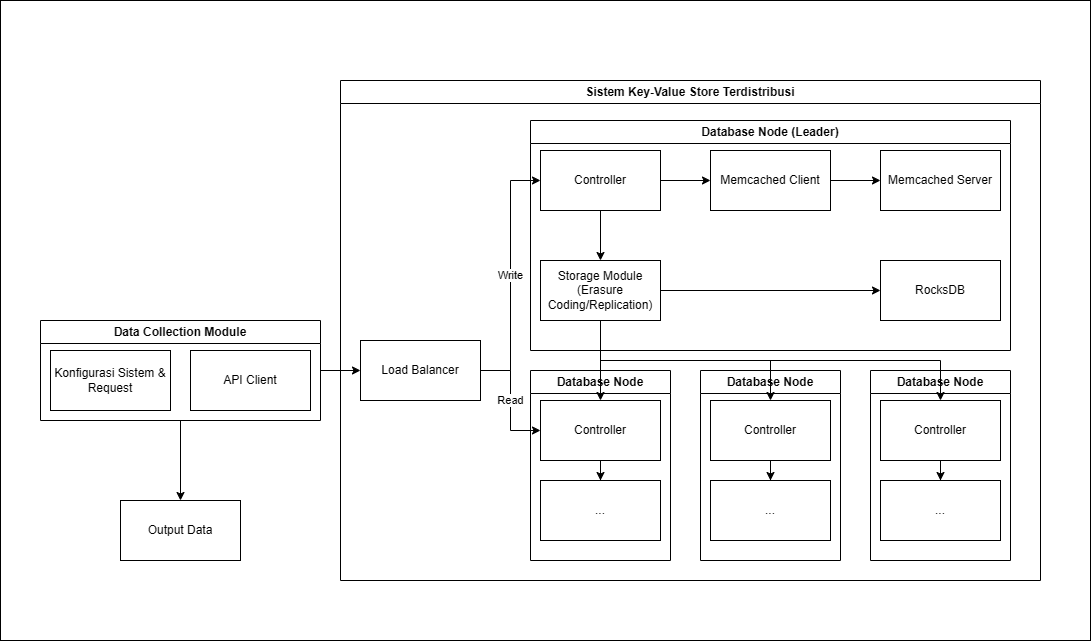
\includegraphics[width=0.95\textwidth]{resources/chapter-3/general-architecture.png}
    \caption{Gambaran Arsitektur Sistem Eksperimen}
    \label{fig:general-architecture}
\end{figure}

Arsitektur dari sistem mengasumsikan kebutuhan untuk konsistensi yang tinggi. Untuk mencapai konsistensi tersebut, operasi \textit{write} dilakukan secara \textit{synchronous} dengan distribusi replikasi dan \textit{erasure coding} dianggap selesai ketika nilai ketahanan yang diinginkan sudah tercapai.

Karena sistem bersifat terdistribusi, maka diperlukan sebuah algoritma konsensus untuk mengelola konsistensi antar \textit{Node}. Algoritma konsensus yang digunakan algoritma konsensus \textit{paxos} yang disesuaikan dengan kebutuhan. Salah satu penyesuaian yang dilakukan adalah mengadopsi pola \textit{leader-follower} untuk memudahkan sinkronisasi data dan mempercepat transaksi. Dengan adanya leader, fase 1 dari algoritma \textit{paxos} dapat dihilangkan dengan membuat proposal dari leader selalu memiliki nilai paling tinggi. Detail implementasi \textit{paxos} akan dijelaskan di bagian \ref{subsection:detail-komponen}. Diagram gambaran arsitektur sistem dapat dilihat pada gambar \ref{fig:general-architecture}.

Operasi \textit{write} akan secara ekslusif disalurkan pada \textit{leader}. Kemudian untuk ketahanan, data akan didistribusikan pada \textit{follower} sesuai dengan konfigurasi \textit{node}. Sementara itu, operasi \textit{read} dapat dilakukan pada \textit{Node} manapun. Pada sistem \textit{erasure coding}, jika pada \textit{node} tersebut tidak terdapat nilai data yang dicari, maka \textit{Node} akan melakukan \textit{request} ke semua node lainnya untuk melakukan rekonstruksi data.

\subsection{Alur Transaksi}
\label{subsection:system-flow}

Alur untuk transaksi \textit{read} dapat dilihat pada gambar \ref{fig:flow-read-mermaidjs} dengan \textit{request} masuk ke \textit{load balancer} kemudian disalurkan ke \textit{database node} yang tersedia. \textit{Database node} akan melakukan operasi \textit{read} pada \textit{key-value store} dan mengembalikan hasil operasi ke \textit{load balancer} untuk dikirimkan ke \textit{client} jika tersedia. Jika tidak, maka \textit{database node} akan melakukan rekonstruksi data dari \textit{erasure-coded persistent data} yang tersebar pada \textit{node-node} lainnya. Pada replikasi, data akan diambil dari \textit{node} lain yang memiliki data yang sama.

\begin{figure}[!ht]
    \centering
    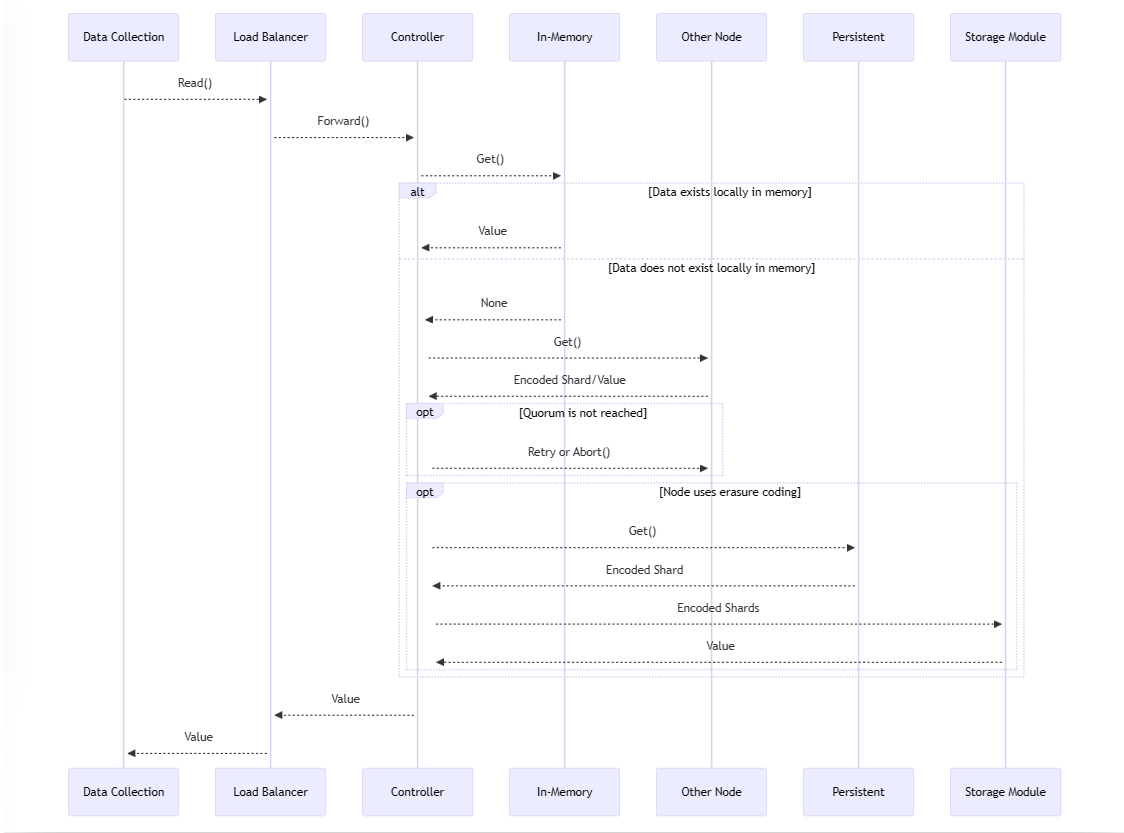
\includegraphics[width=0.95\textwidth]{resources/chapter-3/flow-read-mermaidjs.png}
    \caption{Flow operasi \textit{read} dalam rancangan implementasi}
    \label{fig:flow-read-mermaidjs}
\end{figure}

Alur untuk transaksi \textit{read} dapat dilihat pada gambar \ref{fig:flow-write-mermaidjs} dengan \textit{request} masuk ke \textit{load balancer} kemudian disalurkan ke \textit{database node} yang merupakan leader. Leader kemudian akan melakukan operasi \textit{erasure coding} lalu menyebarkan \textit{shard} ke \textit{follower} yang tersedia. Setelah semua \textit{follower} menerima \textit{shard}, maka operasi \textit{write} dianggap selesai. Operasi \textit{write} pada replikasi juga akan menunggu semua \textit{follower} menerima data sebelum dianggap selesai. 

\begin{figure}[!ht]
    \centering
    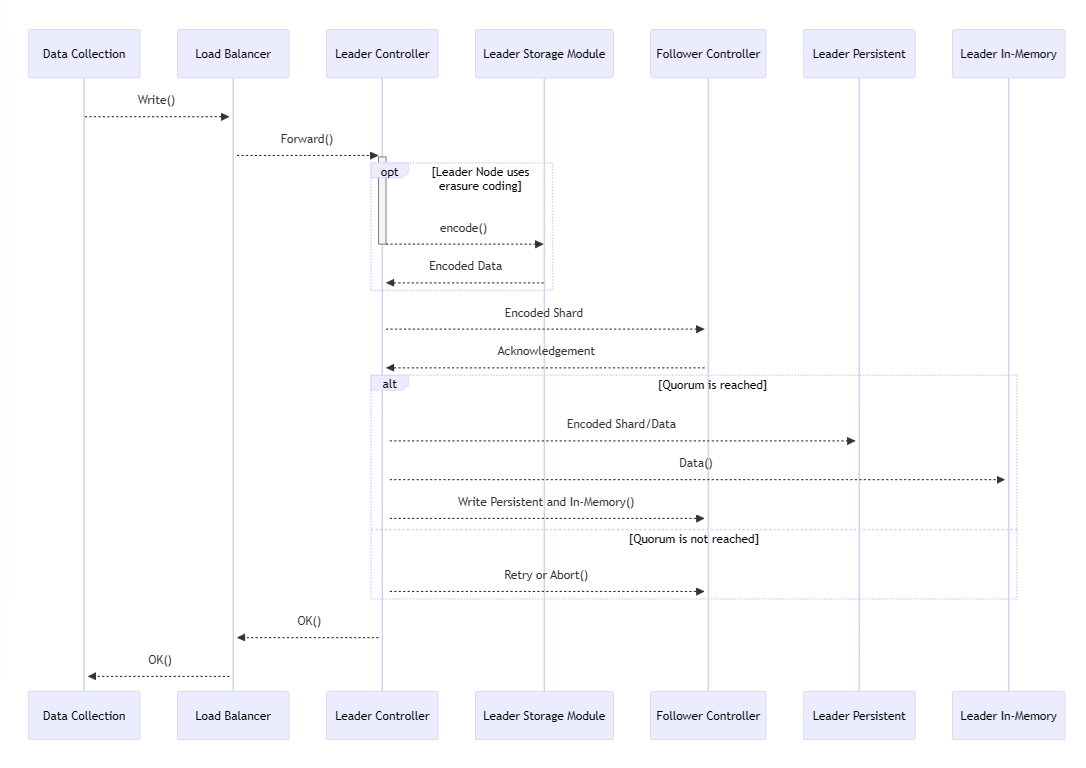
\includegraphics[width=0.95\textwidth]{resources/chapter-3/flow-write-mermaidjs.png}
    \caption{Flow operasi \textit{write} dalam rancangan implementasi}
    \label{fig:flow-write-mermaidjs}
\end{figure}

\subsection{Rancangan Detail Komponen}
\label{subsection:detail-komponen}

Berdasarkan rancangan struktural yang sudah dijelaskan pada bagian \ref{subsection:rancangan-struktural}, sistem akan diimplementasikan sebagai kumpulan komponen. Masing-masing komponen tersebut memiliki peran dan tanggung jawab yang berbeda dalam sistem eksperimen. Pada bagian ini, akan dijelaskan lebih lanjut mengenai rancangan detail dari masing-masing komponen tersebut.

\subsection{Rancangan Detail Node}
\label{subsection:detail-node}

Seperti yang sudah dijelaskan pada bagian \ref{sec:rancangan-struktural}, \textit{Node} merupakan satuan fungsional utama yang berperan sebagai entitas dalam sistem \textit{database} terdistribusi yang dikembangkan.

Struktur \textit{Node} terdiri dari:

\begin{enumerate}
    \item Subsistem penyimpanan: Subsistem ini bertanggung jawab untuk fungsionalitas \textit{key-value store} dalam sebuah \textit{Node}. Detail dari subsistem penyimpanan akan dijelaskan pada bagian \ref{subsection:detail-subsistem-penyimpanan}.
    \item Subsistem kontrol: Subsistem ini bertanggung jawab mengelola transaksi dan konsistensi antar-\textit{Node}. Detail dari subsistem kontrol akan dijelaskan pada bagian \ref{subsection:detail-subsistem-kontrol}.
    \item Komponen HTTP \textit{server}: Komponen ini berperan sebagai antarmuka komunikasi antara \textit{client} dan \textit{Node}. Detail dari komponen HTTP \textit{server} akan dijelaskan pada bagian \ref{subsection:detail-komponen-HTTP-server}.
    \item Komponen komunikasi antar-\textit{Node}: Komponen ini berfungsi untuk mengelola komunikasi antar-\textit{Node} dalam sistem terdistribusi. Detail dari komponen komunikasi antar-\textit{Node} akan dijelaskan pada bagian \ref{subsection:detail-subsistem-komunikasi-antar-node}.
\end{enumerate}

Ilustrasi struktur \textit{Node} dapat dilihat pada gambar \ref{fig:node-structure}.

% _TODO: Change image
\begin{figure}[ht]
    \centering
    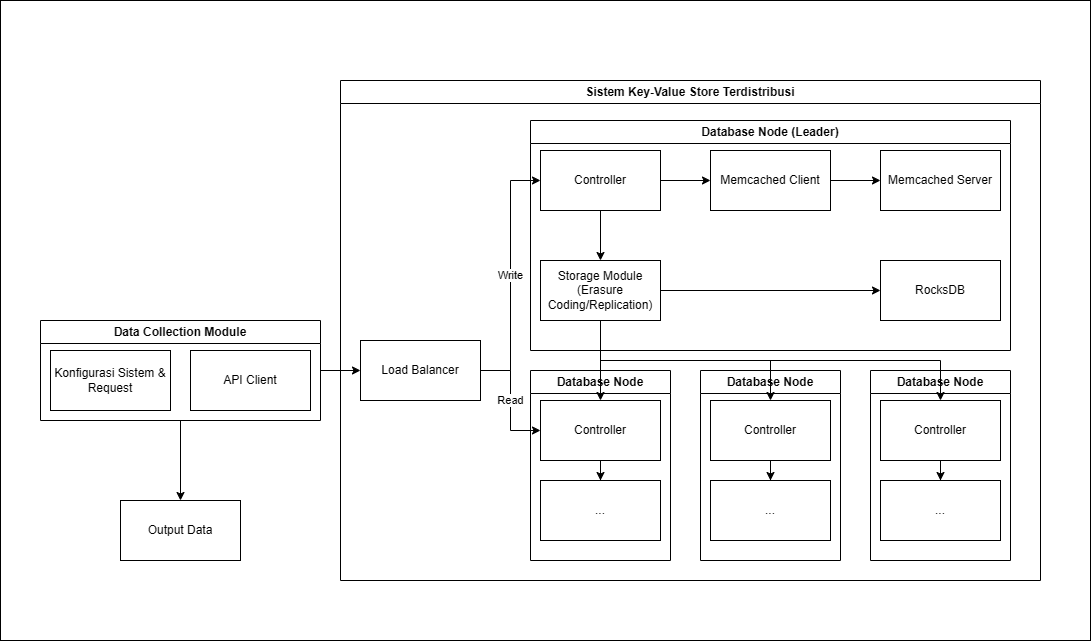
\includegraphics[width=0.95\textwidth]{resources/chapter-3/general-architecture.png}
    \caption{Struktur Node}
    \label{fig:node-structure}
\end{figure}
\subsubsection{Rancangan Detail Subsistem Penyimpanan}
\label{subsubsection:detail-subsistem-penyimpanan}

Subsistem penyimpanan adalah subsistem yang bertanggung jawab untuk fungsionalitas \textit{key-value store} dalam sebuah \textit{Node}. Subsistem ini akan terdiri atas komponen \textit{in-memory store}, \textit{persistent store}, \textit{transaction log}. Subsistem ini juga mengkonfigurasi \textit{Node} untuk menggunakan replikasi atau \textit{erasure coding}.

Mengikuti solusi yang sudah dipilih pada bagian \ref{sec:alternatif-solusi}, subsistem penyimpanan bersifat modular dengan Memcached sebagai \textit{in-memory key-value store} dan RocksDB sebagai \textit{persistent storage}. Memcached memiliki struktur \textit{server} dan \textit{client} sehingga subsistem ini berisi \textit{client} Memcached untuk berkomunikasi dengan \textit{server}. Pada rancangannya, dalam satu perangkat akan dijalankan satu \textit{server} Memcached untuk tiap \textit{Node} yang ada. Sementara itu, RocksDB dapat dijalankan pada tiap node tanpa memerlukan \textit{server}.

Ilustrasi struktur subsistem penyimpanan dapat dilihat pada gambar \ref{fig:storage-subsystem-structure}.

% _TODO: Change image
\begin{figure}[ht]
    \centering
    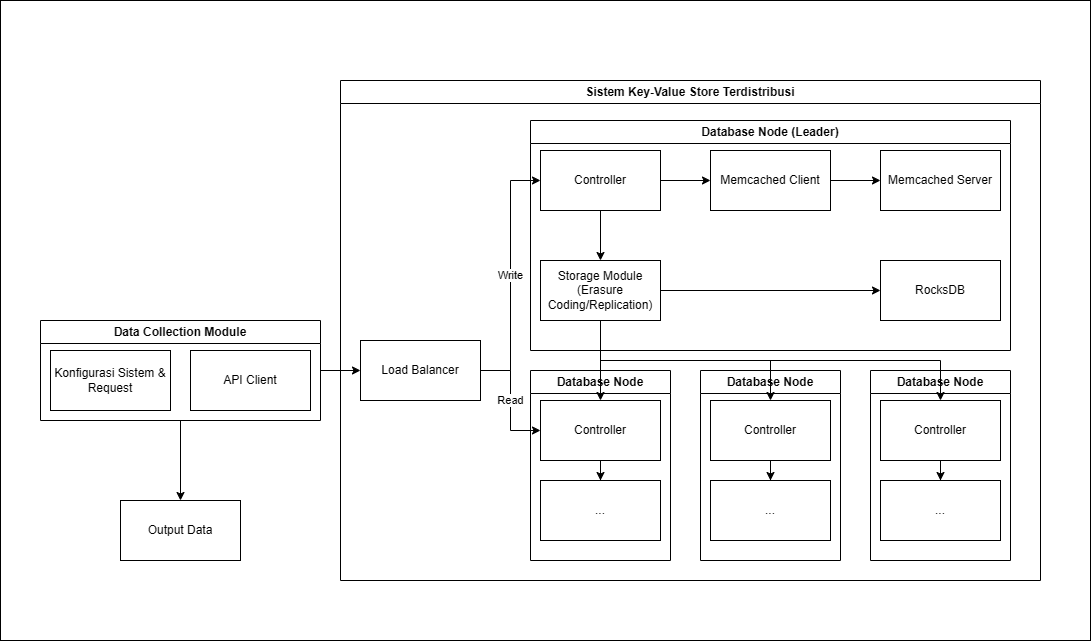
\includegraphics[width=0.95\textwidth]{resources/chapter-3/general-architecture.png}
    \caption{Struktur Subsistem Penyimpanan}
    \label{fig:storage-subsystem-structure}
\end{figure}

\subsubsection{Rancangan Detail Subsistem Kontrol}
\label{subsubsection:detail-subsistem-kontrol}
\subsubsection{Rancangan Detail Komponen HTTP Server}
\label{subsubsection:detail-komponen-HTTP-server}

Komponen HTTP \textit{server} berfungsi sebagai antarmuka komunikasi antara \textit{client} dan \textit{Node}. Komponen ini bertanggung jawab untuk menerima dan memproses permintaan dari \textit{client}, serta mengirimkan respons yang sesuai.

Ilustrasi struktur komponen HTTP \textit{server} dapat dilihat pada gambar \ref{fig:http-server-structure}.

% _TODO: Change image
\begin{figure}[ht]
    \centering
    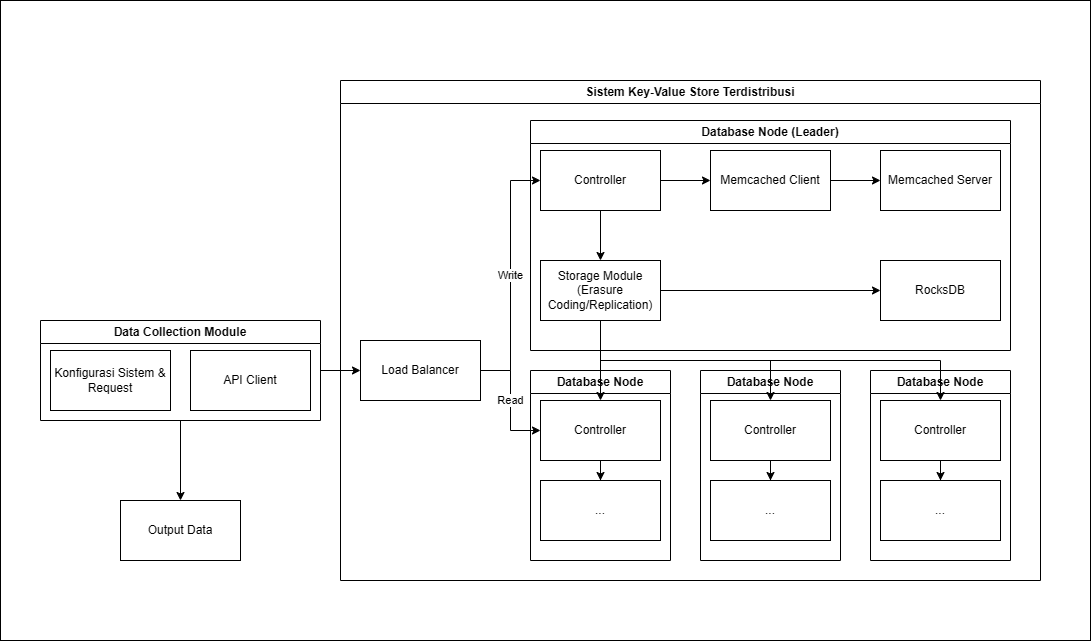
\includegraphics[width=0.95\textwidth]{resources/chapter-3/general-architecture.png}
    \caption{Struktur Komponen HTTP Server}
    \label{fig:http-server-structure}
\end{figure}

\subsubsection{Rancangan Detail Komponen Komunikasi Antar-Node}
\label{subsubsection:detail-subsistem-komunikasi-antar-node}

Komponen komunikasi antar-\textit{Node} bertanggung jawab untuk mengelola komunikasi antar-\textit{Node} dalam sistem terdistribusi. Komponen ini akan menggunakan protokol komunikasi yang sesuai untuk memastikan bahwa data dapat dikirim dan diterima.

Ilustrasi struktur komponen komunikasi antar-\textit{Node} dapat dilihat pada gambar \ref{fig:node-communication-structure}.

% _TODO: Change image
\begin{figure}[ht]
    \centering
    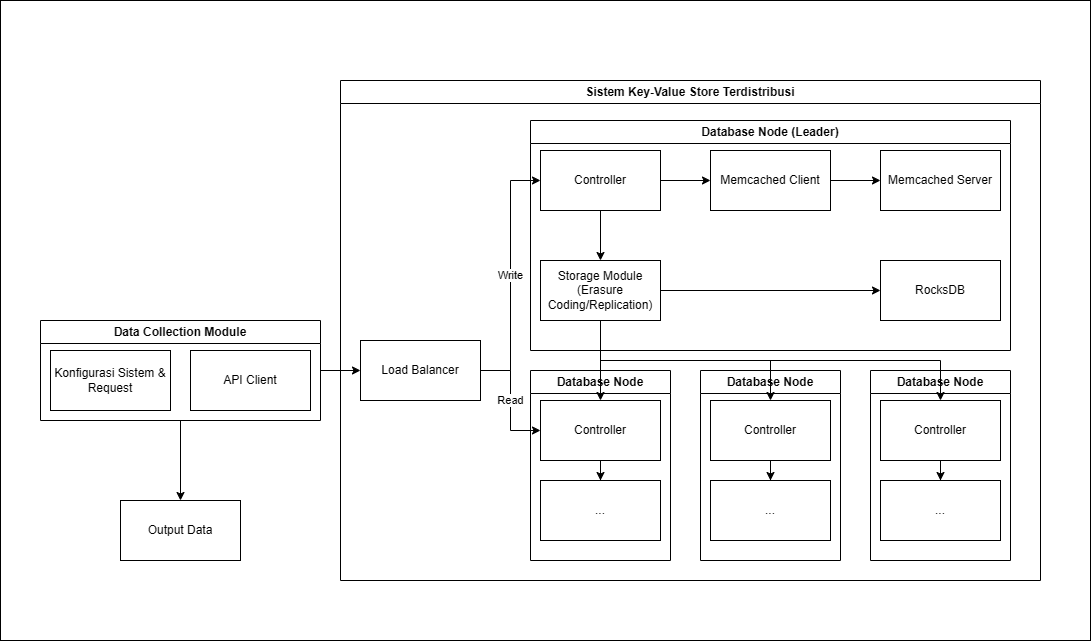
\includegraphics[width=0.95\textwidth]{resources/chapter-3/general-architecture.png}
    \caption{Struktur Komponen Komunikasi Antar-Node}
    \label{fig:node-communication-structure}
\end{figure}
\subsection{Rancangan Detail Data Collector}
\label{subsection:detail-data-collector}

Data Collector adalah komponen yang bertanggung jawab untuk mengumpulkan data dari sistem dan menyimpannya dalam format yang sesuai untuk analisis lebih lanjut. Komponen ini akan mengumpulkan data dari berbagai sumber, termasuk log sistem, metrik kinerja, dan informasi lainnya yang relevan.
Data Collector juga akan menyediakan antarmuka untuk mengakses data yang telah dikumpulkan, sehingga memudahkan pengguna untuk melakukan analisis dan visualisasi data.

Struktur \textit{Data Collector} terdiri dari:

\begin{enumerate}
    \item Komponen testing: Komponen ini bertanggung jawab untuk melakukan \textit{request} dan transaksi pada sistem.
    \item Komponen \textit{logging} dan \textit{tracing}: Komponen ini mengelola pencatatan dan pelacakan operasi yang dilakukan oleh sistem secara keseluruhan.
    \item Komponen \textit{reporting}: Komponen ini bertanggung jawab untuk mengumpulkan dan menyajikan hasil eksperimen dalam bentuk laporan.
\end{enumerate}

Ilustrasi struktur Data Collector dapat dilihat pada gambar \ref{fig:data-collector-structure}.

% _TODO: Change image
\begin{figure}[ht]
    \centering
    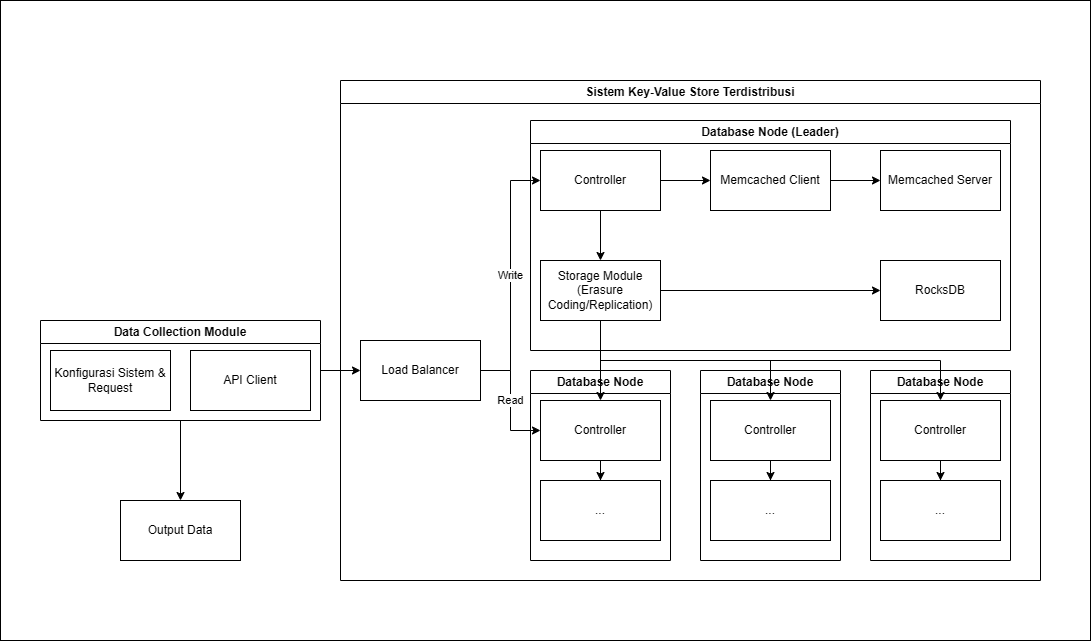
\includegraphics[width=0.95\textwidth]{resources/chapter-3/general-architecture.png}
    \caption{Struktur Data Collector}
    \label{fig:data-collector-structure}
\end{figure}
\subsubsection{Rancangan Detail Komponen Testing}
\label{subsubsection:detail-data-collector}

Komponen \textit{testing} bertanggung jawab untuk melakukan pengujian terhadap sistem yang telah dibangun. Pengujian ini dilakukan untuk memastikan bahwa sistem berfungsi sesuai dengan spesifikasi yang telah ditentukan. Komponen ini juga bertanggung jawab untuk menghasilkan data yang kemudian dimasukkan ke komponen \textit{reporting} untuk visualisasi dan analisis.

Ilustrasi struktur komponen \textit{testing} dapat dilihat pada gambar \ref{fig:testing-structure}.

% _TODO: Change image
\begin{figure}[ht]
    \centering
    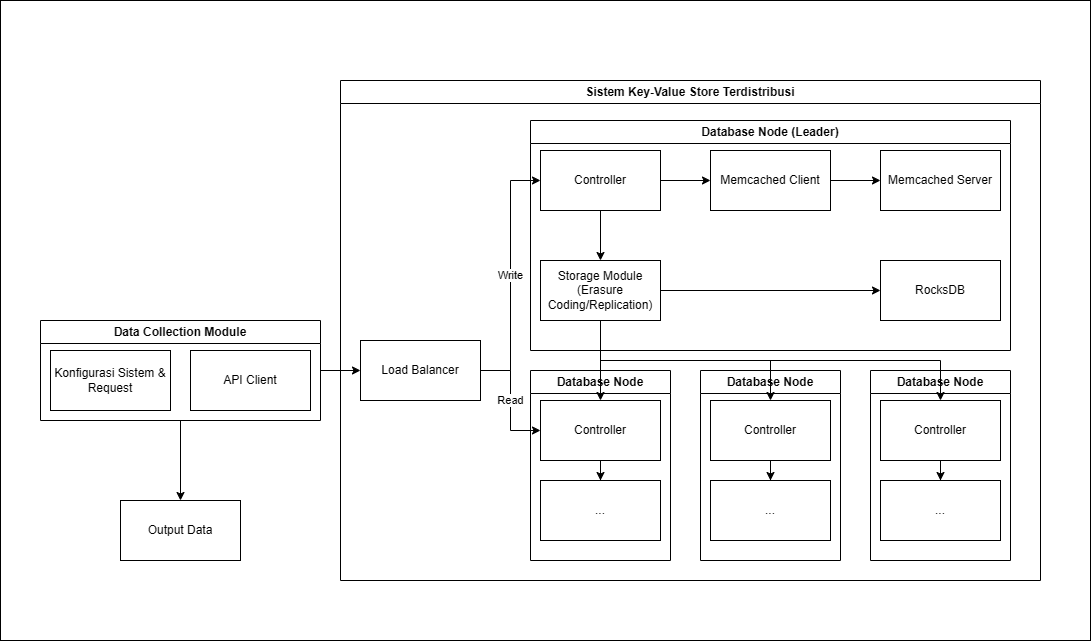
\includegraphics[width=0.95\textwidth]{resources/chapter-3/general-architecture.png}
    \caption{Struktur Komponen Testing}
    \label{fig:testing-structure}
\end{figure}
\subsubsection{Rancangan Detail Komponen Logging dan Tracing}
\label{subsubsection:detail-data-collector}

Komponen \textit{logging} dan \textit{tracing} bertanggung jawab untuk mencatat dan melacak aktivitas sistem. Komponen ini akan mengumpulkan data dari berbagai komponen lain dalam sistem, termasuk informasi tentang permintaan yang diterima, respons yang dikirim, dan status sistem secara keseluruhan. Data ini akan digunakan untuk analisis lebih lanjut dan pemecahan masalah.

Ilustrasi struktur komponen \textit{logging} dan \textit{tracing} dapat dilihat pada gambar \ref{fig:logging-tracing-structure}.

% _TODO: Change image
\begin{figure}[ht]
    \centering
    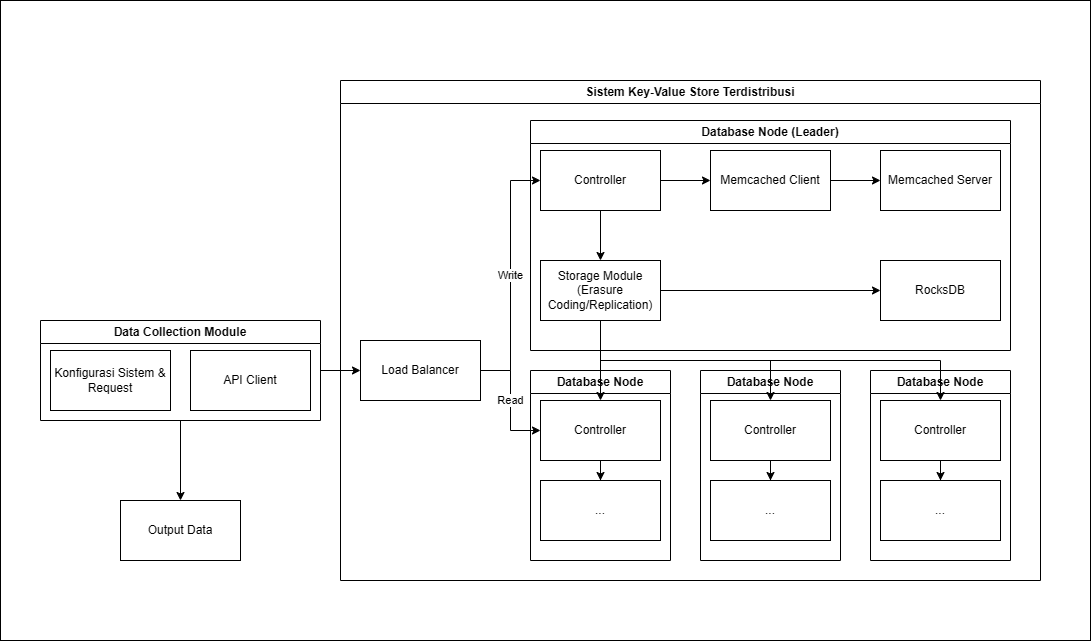
\includegraphics[width=0.95\textwidth]{resources/chapter-3/general-architecture.png}
    \caption{Struktur Komponen Logging dan Tracing}
    \label{fig:logging-tracing-structure}
\end{figure}
\subsubsection{Rancangan Detail Komponen Reporting}
\label{subsubsection:detail-reporting}

Komponen \textit{reporting} bertanggung jawab untuk menghasilkan laporan berdasarkan data yang telah dikumpulkan oleh komponen \textit{data collector}. Komponen ini akan memproses data dan menghasilkan visualisasi yang dapat digunakan untuk analisis lebih lanjut.

Ilustrasi struktur komponen \textit{reporting} dapat dilihat pada gambar \ref{fig:reporting-structure}.

% _TODO: Change image
\begin{figure}[ht]
    \centering
    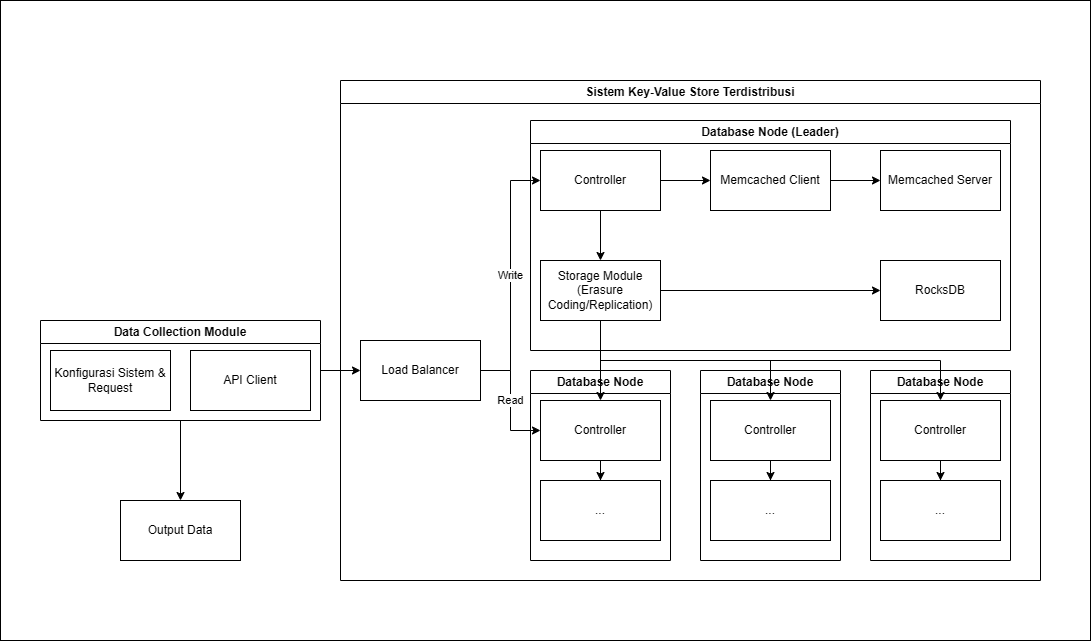
\includegraphics[width=0.95\textwidth]{resources/chapter-3/general-architecture.png}
    \caption{Struktur Komponen Reporting}
    \label{fig:reporting-structure}
\end{figure}

